\documentclass[10pt,a4paper,twocolumn]{article}
\usepackage[utf8]{inputenc}
\usepackage[T1]{fontenc}
\usepackage[spanish,es-tabla]{babel}
\usepackage[margin=1.6cm,columnsep=0.7cm]{geometry}
\usepackage{graphicx,booktabs,xcolor,microtype}
\usepackage{enumitem}
\usepackage[font=footnotesize,skip=2pt]{caption}
\usepackage{titlesec}
\usepackage{float}
\titleformat{\subsection}{\normalfont\normalsize\bfseries}{\thesubsection.}{0.5em}{}
\titlespacing*{\subsection}{0pt}{5pt}{2pt}
\usepackage[hidelinks]{hyperref}

\titleformat{\section}{\normalfont\large\bfseries}{\thesection.}{0.5em}{}
\titlespacing*{\section}{0pt}{8pt}{3pt}
\setlist{nosep,leftmargin=1.2em}

% Marcas rojas para completar (desaparecen al reemplazarlas)
\newcommand{\TODO}[1]{\textcolor{red}{[#1]}}
\newcommand{\refx}[1]{\textcolor{red}{[ref: #1]}}   % reemplazar por \cite{clave}

\title{\bfseries Comparación de arquitecturas de ingesta (Lambda y Kappa)\\
y de API (REST y GraphQL): un benchmark de rendimiento}
\author{Katia Daishy Ticona Casa\\
\small Maestría en Informática, Mención en Gerencia de TIC -- Universidad Nacional del Altiplano de Puno\\
\small Curso: Business Intelligence \quad k.ticona@est.unap.edu.pe}
\date{Octubre de 2026}

\begin{document}
\maketitle

\begin{abstract}\small
Se implementó una plataforma de ingesta de eventos con dos arquitecturas (Lambda y Kappa) y dos estilos de API
(REST y GraphQL) sobre una misma base de datos, y se midió su rendimiento. Kappa tuvo menor latencia p95 que
Lambda en todas las tasas (0.49 frente a 0.79 s con 5\,000 e/s) con throughput equivalente. GraphQL redujo 43\,\%
los bytes por dashboard, pero REST atendió más dashboards por segundo con 10 y 200 usuarios.
\end{abstract}

\section{Introducción}
El análisis de datos casi en tiempo real exige arquitecturas de ingesta que combinen baja latencia y exactitud.
La arquitectura Lambda separa una capa batch, que recalcula las vistas desde un conjunto maestro inmutable,
de una capa speed incremental \cite{demirezen2023}; la arquitectura Kappa trata todos los datos como un flujo y
reprocesa repitiendo el registro de eventos \cite{feick2018,sanla2019}. Sobre estas vistas, las aplicaciones de inteligencia
de negocios consumen datos mediante APIs: REST y GraphQL difieren en el número de peticiones y en la cantidad
de datos transferidos \cite{mikula2020,elghazal2025,seabra2019}. Este trabajo implementa ambas arquitecturas de ingesta y ambos
estilos de API en una plataforma común, y compara su rendimiento con un protocolo reproducible
\cite{karimov2018}.

\section{Plataforma y arquitecturas}
Un generador publica eventos sintéticos en formato JSON (consulta, trámite, pago y reclamo; semilla fija) en
un tópico de Redpanda, compatible con Kafka. Ambas arquitecturas agregan por minuto y tipo de evento, y
escriben en PostgreSQL.

\textbf{Kappa.} Un único consumidor en streaming acumula conteos y montos y los escribe con \emph{upsert} en
una vista; el \emph{offset} se confirma solo después de escribir en la base. Reprocesar equivale a leer el
tópico desde el inicio con un nuevo grupo de consumo.

\textbf{Lambda.} La capa speed guarda cada evento crudo (deduplicado por identificador) y actualiza una vista
incremental en la misma transacción. La capa batch, cada 15 s, recalcula la vista completa desde los datos
crudos y descuenta de la vista speed lo ya cubierto. Una vista de servicio une ambas capas.

\textbf{APIs.} REST (FastAPI) y GraphQL (Strawberry sobre FastAPI) comparten la misma capa de acceso a datos
y el mismo \emph{pool} de conexiones. Ofrecen dos consultas: \emph{resumen} (eventos, monto y promedio por tipo)
y \emph{serie} (eventos y monto por minuto). Ambas pueden leer de la vista Kappa o de la vista de servicio Lambda.

\section{Metodología}
\textbf{Entorno.} \TODO{CPU, núcleos, RAM, sistema operativo, versión de Docker Desktop, versión de Python y
de FastAPI/Strawberry/Locust (usar \texttt{pip freeze})}. Redpanda v24.2.7 y PostgreSQL 16 en contenedores,
una partición de Redpanda y un único trabajador por capa.

\textbf{Ingesta.} Tasas de 500, 2\,000 y 5\,000 eventos/s durante 30 s (15\,000, 60\,000 y 150\,000 eventos),
con 3 repeticiones independientes que alternan arquitecturas; cada corrida usa un tópico y tablas limpios.
\emph{Latencia} es el tiempo entre la producción de un evento y su visibilidad en la vista de consulta
(sondeo cada 100 ms sobre una muestra de unos 3\,000 eventos por corrida); \emph{throughput} es eventos
visibles dividido por el tiempo total hasta que todos lo son; también se midió CPU y memoria (RSS) de los
trabajadores cada 0,5 s y el tiempo de reprocesar 150\,000 eventos desde cero. Ambas arquitecturas escriben
cada 1 s, lo que fija un piso de latencia común. \TODO{Confirmar: se verificó que ambas vistas producen
resultados idénticos (0 diferencias en N claves).}

\textbf{API.} Un \emph{dashboard} es la carga de una pantalla que requiere \emph{resumen} y \emph{serie}:
2 peticiones HTTP en REST y 1 en GraphQL, que solicita solo los campos necesarios, mientras que REST devuelve
el recurso completo. Con Locust se simularon 10, 50 y 200 usuarios concurrentes sin tiempo de espera durante
40 s, 3 repeticiones, contra un servidor \texttt{uvicorn} de un proceso; se registró dashboards/s, latencia
p50/p95/p99 del dashboard completo, bytes por respuesta, fallos, CPU y memoria. Se reportan media $\pm$
desviación estándar de $n=3$.

\section{Resultados}
\subsection{Ingesta: Kappa frente a Lambda}
Con 500, 2\,000 y 5\,000 eventos/s, ambas arquitecturas procesaron todos los eventos en las nueve corridas
de cada una y sostuvieron un throughput cercano a la carga ofrecida (Tabla~\ref{tab:ingesta}). Kappa obtuvo
menor latencia p95 que Lambda en todas las tasas: 1.10 s frente a 1.23 s con 500 e/s, 1.07 s frente a 1.30 s
con 2\,000 e/s y 0.49 s frente a 0.79 s con 5\,000 e/s (Fig.~\ref{fig:lat}).

\begin{table*}[t]\centering\small
\caption{Ingesta: Kappa vs Lambda (media $\pm$ desviación estándar; Compl. = corridas que procesaron todos los eventos).}
\label{tab:ingesta}
\begin{tabular}{rlrrrrrrr}
\toprule
Tasa (e/s) & Arq. & Throughput (e/s) & p50 (s) & p95 (s) & p99 (s) & CPU (\%) & RAM (MB) & n \\
\midrule
500 & Kappa & $484\pm4$ & $0.65\pm0.03$ & $1.11\pm0.04$ & $1.18\pm0.04$ & $3.5\pm2.5$ & $37\pm1$ & 3 \\
 & Lambda & $488\pm7$ & $0.70\pm0.01$ & $1.18\pm0.01$ & $1.26\pm0.03$ & $4.2\pm2.2$ & $62\pm2$ & 3 \\
\midrule
2\,000 & Kappa & $1929\pm2$ & $0.61\pm0.01$ & $1.06\pm0.01$ & $1.13\pm0.02$ & $7.0\pm2.8$ & $35\pm1$ & 3 \\
 & Lambda & $1974\pm2$ & $0.77\pm0.03$ & $1.23\pm0.02$ & $1.30\pm0.02$ & $9.4\pm3.9$ & $58\pm7$ & 3 \\
\midrule
5\,000 & Kappa & $4875\pm16$ & $0.31\pm0.00$ & $0.51\pm0.00$ & $0.86\pm0.10$ & $6.2\pm0.8$ & $36\pm1$ & 3 \\
 & Lambda & $4838\pm4$ & $0.44\pm0.01$ & $0.64\pm0.01$ & $1.09\pm0.02$ & $14.7\pm1.8$ & $64\pm1$ & 3 \\
\midrule
10\,000 & Kappa & $9683\pm43$ & $0.18\pm0.00$ & $0.30\pm0.00$ & $0.34\pm0.02$ & $14.8\pm0.9$ & $34\pm2$ & 3 \\
 & Lambda & $9441\pm274$ & $1.22\pm1.38$ & $1.58\pm1.48$ & $1.69\pm1.47$ & $32.4\pm5.1$ & $66\pm1$ & 3 \\
\midrule
20\,000 & Kappa & $19283\pm7$ & $0.14\pm0.01$ & $0.24\pm0.01$ & $0.35\pm0.10$ & $29.9\pm7.5$ & $34\pm2$ & 3 \\
 & Lambda & $11517\pm996$ & $16.12\pm4.26$ & $20.98\pm4.56$ & $21.30\pm4.63$ & $32.0\pm1.3$ & $100\pm3$ & 3 \\
\bottomrule
\end{tabular}
\end{table*}

\begin{figure}[H]\centering
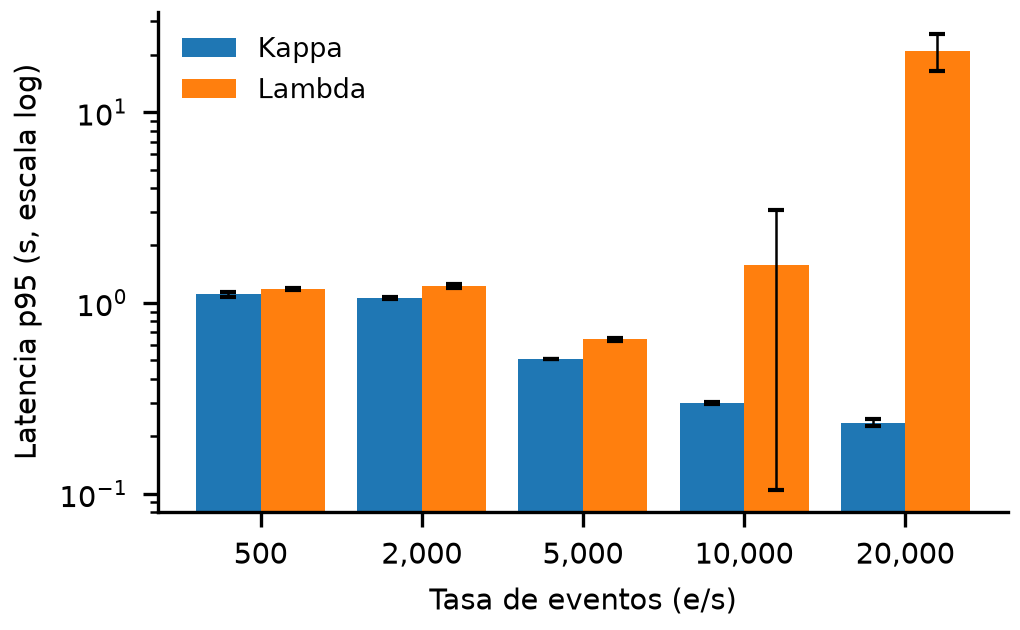
\includegraphics[width=\columnwidth]{fig_ingesta_latencia.png}
\caption{Latencia p95 de la ingesta según la tasa de eventos (media y desviación estándar, $n=3$).}
\label{fig:lat}
\end{figure}

\subsection{API: REST frente a GraphQL}
El dashboard transfirió 667 B en REST (2 peticiones) y 379 B en GraphQL (1 petición), un 43\,\% menos, y no
hubo fallos en ninguna corrida (Tabla~\ref{tab:api}). REST atendió más dashboards por segundo con 10 usuarios
(29.9 frente a 20.2) y con 200 (44.8 frente a 27.2); con 50 usuarios la diferencia fue pequeña (37.6 frente a
35.3) y la latencia p95 coincidió (2.4 s), sin diferencia concluyente con tres repeticiones (Fig.~\ref{fig:rps}).
Con 200 usuarios, que no esperan entre peticiones, el servidor operó saturado y la latencia p95 fue de 8.7 s
en REST y 12.0 s en GraphQL.

\begin{table*}[t]\centering\small
\caption{API: REST vs GraphQL (dashboard = resumen + serie; Bytes = tamaño medio de la respuesta del dashboard).}
\label{tab:api}
\begin{tabular}{rlrrrrrr}
\toprule
Usuarios & API & Dashboards/s & p50 (ms) & p95 (ms) & p99 (ms) & Bytes & Fallos \\
\midrule
10 & GraphQL & $20.2\pm0.9$ & $467\pm21$ & $673\pm40$ & $3067\pm153$ & $379\pm0$ & 0 \\
 & REST & $29.9\pm2.0$ & $280\pm20$ & $523\pm42$ & $950\pm260$ & $667\pm0$ & 0 \\
\midrule
50 & GraphQL & $35.3\pm1.6$ & $1200\pm0$ & $2433\pm289$ & $5033\pm58$ & $379\pm0$ & 0 \\
 & REST & $37.6\pm4.9$ & $1093\pm110$ & $2433\pm351$ & $5100\pm361$ & $667\pm0$ & 0 \\
\midrule
200 & GraphQL & $27.2\pm3.5$ & $6367\pm1124$ & $11967\pm1790$ & $13333\pm2082$ & $379\pm0$ & 0 \\
 & REST & $44.8\pm1.3$ & $3667\pm58$ & $8700\pm700$ & $9400\pm557$ & $667\pm0$ & 0 \\
\bottomrule
\end{tabular}
\end{table*}

\begin{figure}[H]\centering
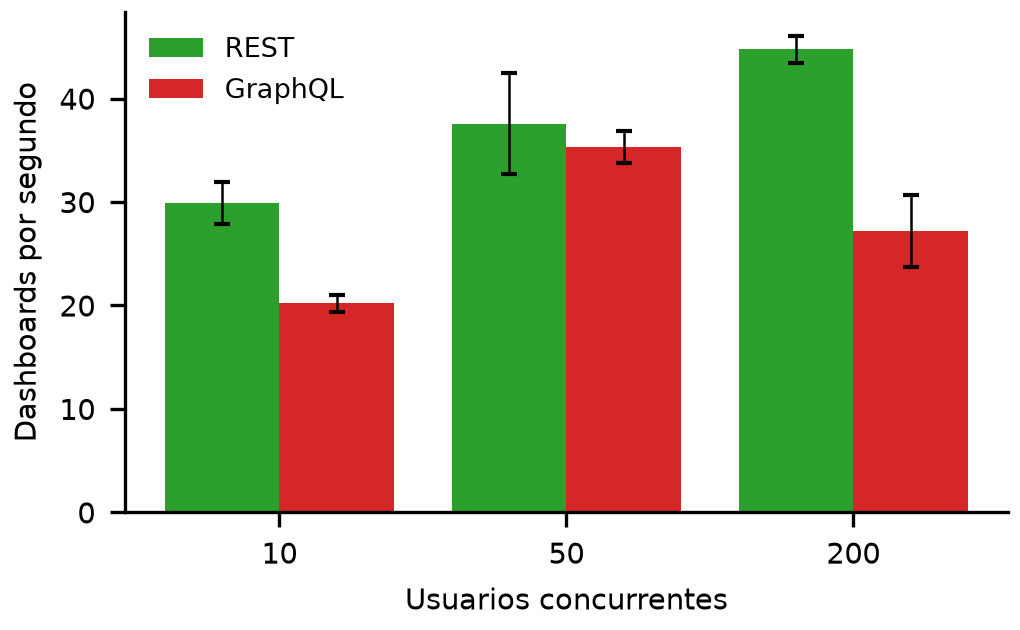
\includegraphics[width=\columnwidth]{fig_api_rps.png}
\caption{Dashboards por segundo según el número de usuarios concurrentes.}
\label{fig:rps}
\end{figure}

\section{Discusión}
\section{Discusión}
La menor latencia de Kappa va en la misma dirección que lo reportado al comparar ambas arquitecturas
\cite{sanla2019}. En las APIs, la mayor tasa de REST bajo carga alta coincide con \cite{elghazal2025} y con la
caída de GraphQL en cargas elevadas de \cite{seabra2019}, mientras que \cite{mikula2020} halló lo contrario con
porciones pequeñas de datos: el resultado depende de la implementación y del tamaño de la respuesta.

\textbf{Limitaciones.} Todo corrió en una sola computadora (generador, trabajadores, Redpanda, PostgreSQL y
Locust compiten por recursos), por lo que los valores sirven para comparar entre configuraciones y no como
valores absolutos; hay una partición, un trabajador por capa, y solo 3 repeticiones por configuración.

\section{Conclusiones}
Se implementó una plataforma reproducible que ingesta eventos con las arquitecturas Kappa y Lambda y los
expone mediante APIs REST y GraphQL sobre la misma base de datos; ambas arquitecturas produjeron los mismos
resultados agregados. En la ingesta, Kappa tuvo menor latencia p95 que Lambda en todas las tasas evaluadas
(500 a 5\,000 eventos/s), con diferencias de 11\,\% a 38\,\%, y ambas sostuvieron la carga ofrecida sin
diferencias relevantes de throughput. Lambda añade una capa batch que recalcula las vistas desde el conjunto
maestro, lo que aporta capacidad de corrección a cambio de más componentes y mayor latencia. En las APIs,
GraphQL redujo 43\,\% los bytes por dashboard (379 frente a 667 B) y las peticiones HTTP de dos a una, pero
REST sostuvo más dashboards por segundo con 10 usuarios (cerca de 30 frente a 20) y con 200 (cerca de 45
frente a 27), sin diferencia concluyente con 50. En consecuencia, Kappa resulta preferible cuando
prima la baja latencia con un único \emph{pipeline}; Lambda, cuando se requiere recalcular o corregir
histórico; GraphQL, cuando el ancho de banda es la restricción; y REST, cuando importa la tasa de atención
bajo carga alta. Estos valores provienen de una sola computadora, un trabajador por capa y tres
repeticiones, por lo que sirven para comparar configuraciones y no como capacidad absoluta; como trabajo
futuro quedan varias particiones, un clúster real y motores como Flink o Spark.

El código y los datos crudos están en \url{https://github.com/KatiaTicona/lambda-kappa} (etiqueta v1.0).
\bibliographystyle{ieeetr}
{\footnotesize\bibliography{referencias}}

\end{document}